% !TEX program = lualatex
\documentclass[a4paper,11pt]{jlreq}

\usepackage{luatexja}
\usepackage{luatexja-fontspec}
\usepackage{amsmath,amssymb,mathtools}
\usepackage{graphicx}
\usepackage{array}
\usepackage{booktabs}
\usepackage{hyperref}
\usepackage{xurl}

\hypersetup{colorlinks=true,linkcolor=blue,urlcolor=blue,citecolor=blue}
\newcommand{\E}{\mathbb{E}}
\newcommand{\R}{\mathbb{R}}
\newcommand{\ii}{\mathrm{i}}
\DeclareMathOperator{\RMSE}{RMSE}

\title{一般化Boole写像に対するE0・E1の定式化\\数値実験結果と考察}
\author{長松 蒼空}
\date{2026年9月1日}

\begin{document}
\maketitle

\begin{abstract}
本ノートでは、カオス同期による情報圧縮研究の前段として実施したE0とE1を定式化し、
保存済み数値実験の結果とその解釈可能範囲を整理する。
E0は単一の非結合一般化Boole写像について、Cauchy不変測度、Lyapunov指数、
Cayley冪モードの定常平均を再現し、理論と実装の整合性を検査する実験である。
E1Aでは周辺Cauchy尺度を軌道ごとに除いた後、有限時間特徴から未使用の写像パラメータを回帰した。
最初の48 seed追試ではTM型時間遅延とFourierの差の95\%区間が0を含んだが、
両者を16次元へ揃え、TM座標をfit seedだけで選ぶ容量一致追試では、
TMのtest RMSEは0.001342、Fourierは0.002614となり、差の95\%区間は正だった。
E1Bでは2源へ拡張し、既知の可逆2観測では順序付き2パラメータを回収できる一方、
対称1観測では源入替えにより同一観測へ異なる順序付き目標が対応するため、
RMSEに厳密な下限が生じることを数式と完全衝突データで確認した。
以上は有限時間情報の存在と観測写像の識別可能性境界を支持するが、
同期、blind source separation、rate--distortion、画像復号の成立は未証明である。
\end{abstract}

\section{研究上の位置づけ}

本研究の最終目標は、同期による自由度縮約の中に入力依存情報を残し、
その情報を有限次元表現から復号できる条件を明らかにすることである。
ただし、同期したことと有用な情報圧縮が成立したことは同値ではない。
この混同を避けるため、E0とE1の役割を次のように分離する。

\begin{center}
\begin{tabular}{p{0.12\linewidth}p{0.35\linewidth}p{0.43\linewidth}}
\toprule
段階 & 問うこと & 問わないこと \\
\midrule
E0 & 単一写像の理論式を数値実装が再現するか & 結合、同期、復号、圧縮の有用性 \\
E1 & 軌道に残る既知パラメータを読み出せるか & 同期による自由度縮約、rate--distortion \\
\bottomrule
\end{tabular}
\end{center}

以下では、解析的に既知または原典と照合済みの事項を「理論」、
保存データから確認した事項を「数値観察」、まだ示されていない事項を「未解決」として区別する。

\section{E0：一般化Boole写像の理論・実装整合性}

\subsection{局所写像とCauchy尺度写像}

局所力学として、一般化Boole写像
\begin{equation}
    x_{t+1}=F_{\alpha}(x_t),
    \qquad
    F_{\alpha}(x)=\alpha\left(x-\frac{1}{x}\right),
    \qquad 0<\alpha<1
    \label{eq:boole-map}
\end{equation}
を考える。状態はBoolean値ではなく、$x_t\in\R\setminus\{0\}$ の実数である。

より一般の写像 $T_{\alpha,\beta}(x)=\alpha x-\beta/x$ に
中心0、尺度$\gamma>0$のCauchy密度
\begin{equation}
    \rho_{\gamma}(x)
    =\frac{\gamma}{\pi\left(x^2+\gamma^2\right)}
    \label{eq:cauchy-density}
\end{equation}
を入力すると、Cauchy族の中では尺度が
\begin{equation}
    \gamma_{t+1}
    =G_{\alpha,\beta}(\gamma_t)
    =\alpha\gamma_t+\frac{\beta}{\gamma_t}
    \label{eq:scale-map-general}
\end{equation}
と更新される\cite{umeno2026,umeno2016}。
E0では$\beta=\alpha$なので、
\begin{equation}
    \gamma_{t+1}
    =\alpha\left(\gamma_t+\frac{1}{\gamma_t}\right)
    \label{eq:scale-map}
\end{equation}
である。正の固定点$\gamma_{\ast}$は
\begin{equation}
    \gamma_{\ast}^2=\frac{\alpha}{1-\alpha},
    \qquad
    \gamma_{\ast}=\sqrt{\frac{\alpha}{1-\alpha}}
    \label{eq:fixed-scale}
\end{equation}
となる。また、Cauchy族内の尺度摂動に対して
\begin{equation}
    G'_{\alpha,\alpha}(\gamma_{\ast})
    =\alpha-\frac{\alpha}{\gamma_{\ast}^{2}}
    =2\alpha-1
\end{equation}
であり、$0<\alpha<1$では$|2\alpha-1|<1$である。
これはCauchy族内の固定尺度の局所安定性を示すが、任意の初期分布からの大域収束をこの式だけで保証するものではない。

\subsection{Lyapunov指数}

写像の導関数は
\begin{equation}
    F'_{\alpha}(x)=\alpha\left(1+\frac{1}{x^2}\right)
\end{equation}
である。不変Cauchy密度に関するLyapunov指数は
\begin{align}
    \lambda(\alpha)
    &=\int_{-\infty}^{\infty}
      \rho_{\gamma_{\ast}}(x)
      \log\left|F'_{\alpha}(x)\right|\,\mathrm{d}x \\
    &=\log\alpha
      +2\log\left(1+\frac{1}{\gamma_{\ast}}\right) \\
    &=2\log\left(\sqrt{\alpha}+\sqrt{1-\alpha}\right).
    \label{eq:lyapunov-closed}
\end{align}
この値は$0<\alpha<1$で正であり、$\alpha=1/2$で最大値$\log 2$をとる。
E0は式\eqref{eq:lyapunov-closed}を、軌道平均と独立な角度座標数値積分の二経路で照合する。

\subsection{Cayley冪モード}

尺度$\gamma$に対するCayley変換を
\begin{equation}
    q_{\gamma}(x)=\frac{x-\ii\gamma}{x+\ii\gamma}
    \label{eq:cayley}
\end{equation}
とする。実数$x$に対して$|q_{\gamma}(x)|=1$である。
$X\sim\mathrm{Cauchy}(0,\gamma)$を$X=\gamma\tan\Theta$、
$\Theta\sim\mathrm{Uniform}(-\pi/2,\pi/2)$と書けば、
$q_{\gamma}(X)=-\exp(2\ii\Theta)$となるため、非零整数$k$について
\begin{equation}
    \E\left[q_{\gamma}(X)^k\right]=0
    \label{eq:cayley-moment-zero}
\end{equation}
である。E0で評価する
\begin{equation}
    \widehat c_k
    =\frac{1}{T}\sum_{t=1}^{T}q_{\gamma_{\ast}}(x_t)^k,
    \qquad k=1,\ldots,8
    \label{eq:e0-cayley-coefficient}
\end{equation}
は、完全なTakenaka--Malmquist系そのものではなく、Cayley変換の有限冪モードである。
したがって、式\eqref{eq:cayley-moment-zero}の再現は一般のTM系の完全性や読み出し性能を保証しない。

\subsection{E0の数値実験設計}

使用したパラメータは$\alpha\in\{0.4,0.5,0.6\}$、各5 seedである。
各軌道は理論Cauchy分布から初期化し、20,000点をburn-inした後、100,000点を観測した。
全15軌道、合計1,500,000観測点である。

重い裾を持つCauchy分布では平均と分散が存在しないため、尺度推定には
\begin{equation}
    \widehat\gamma
    =\frac{Q_{0.75}-Q_{0.25}}{2}
    \label{eq:robust-scale}
\end{equation}
を用いた。その他の指標は、理論Cauchy分布とのKolmogorov--Smirnov距離$D_{\mathrm{KS}}$、
有限時間Lyapunov指数
\begin{equation}
    \widehat\lambda_T
    =\frac{1}{T}\sum_{t=1}^{T}\log\left|F'_{\alpha}(x_t)\right|,
\end{equation}
および式\eqref{eq:e0-cayley-coefficient}の最大絶対値である。

事前の工学的合格閾値は、尺度相対誤差$\le 0.05$、Lyapunov絶対誤差$\le 0.015$、
$D_{\mathrm{KS}}\le 0.02$、最大非零Cayleyモード$\le 0.02$、
独立数値積分のLyapunov誤差$\le 10^{-5}$とした。
これらは実装回帰を検出する閾値であり、統計的有意水準ではない。

\subsection{E0の結果}

\begin{table}[htbp]
\centering
\small
\caption{E0の理論値と5 seed中の最大誤差。}
\label{tab:e0-results}
\begin{tabular}{ccccccc}
\toprule
$\alpha$ & $\gamma_{\ast}$ & $\lambda$ & 尺度相対誤差 & Lyapunov誤差 & $D_{\mathrm{KS}}$ & $\max_{k}|\widehat c_k|$ \\
\midrule
0.4 & 0.816497 & 0.682994 & 0.013948 & 0.001175 & 0.006502 & 0.007621 \\
0.5 & 1.000000 & 0.693147 & 0.007904 & 0.000031 & 0.004497 & 0.004496 \\
0.6 & 1.224745 & 0.682994 & 0.007178 & 0.000810 & 0.005901 & 0.006524 \\
\bottomrule
\end{tabular}
\end{table}

全$\alpha$・全seedで、状態は有限値を保ち、100,000点の観測区間に厳密な重複はなかった。
最大誤差はすべて事前閾値内であり、独立角度積分と閉形式Lyapunov指数の最大差は
$6.93\times10^{-6}$だった。保存成果物に対する独立検証は37項目中37項目が通過した。

\subsection{E0の考察}

E0が支持するのは、式\eqref{eq:boole-map}の単一非結合ノードについて、
Cauchy尺度、Lyapunov指数、Cayley冪モードを実装が整合的に再現したという限定的主張である。
$\alpha=0.4$と$0.6$で理論Lyapunov指数が等しく、$\alpha=0.5$で$\log2$になる対称性も再現された。

一方、初期値を理論不変測度から生成しているため、任意の非定常初期分布からの収束速度は未検証である。
観測区間で重複がないことも、より長時間の浮動小数点周期化が存在しない証明ではない。
また、E0には複数ノード、結合、同期誤差、復号、符号長が含まれない。
したがって、E0の成功から情報圧縮やカオス同期エンコーダの有用性を結論してはならない。

\section{E1：有限時間軌道からの読み出し}

\subsection{E1全体と実施済みE1A・E1Bの区別}

E1全体の目的は、既知のクラスタ、位相差、尺度などを持つ人工軌道から、
TM、グラフ、時間遅延特徴によって既知量を復号できる条件と失敗条件を示すことである。
E1Aでは同期結合も線形混合も導入せず、式\eqref{eq:boole-map}の一軌道から$\alpha$を推定する。
続くE1Bでは2本の独立軌道を線形観測し、可逆な2観測と対称な1観測を比較する。
ただし、いずれも同期結合を含まない読み出し単体検証であり、
本節の成功は同期による自由度縮約や圧縮の成立を意味しない。

\subsection{周辺尺度を除いた識別問題}

軌道$r$の観測を$x^{(r)}_1,\ldots,x^{(r)}_T$とする。
まず、軌道ごとの中央値$\widehat m_r$と半四分位幅$\widehat\gamma_r$を用いて
\begin{equation}
    u^{(r)}_t
    =\frac{x^{(r)}_t-\widehat m_r}{\widehat\gamma_r},
    \qquad
    \widehat\gamma_r
    =\frac{Q^{(r)}_{0.75}-Q^{(r)}_{0.25}}{2}
    \label{eq:e1-standardization}
\end{equation}
と標準化する。$\widehat\gamma_r$自体は回帰器へ渡さない。
これにより、理論式\eqref{eq:fixed-scale}が与える周辺尺度だけから$\alpha$を読む自明な経路を抑える。
ただし、有限標本の$\widehat\gamma_r$には推定誤差があるため、周辺情報を完全に消したとは言えない。

標準化系列を尺度1のCayley変換
\begin{equation}
    z^{(r)}_t
    =q_1\!\left(u^{(r)}_t\right)
    =\frac{u^{(r)}_t-\ii}{u^{(r)}_t+\ii}
    \label{eq:e1-cayley}
\end{equation}
で単位円上へ写す。

\subsection{TM型時間遅延特徴と識別条件}

次数$k=1,\ldots,K$の定常平均と、遅延$\tau\in\mathcal T$の相関を
\begin{align}
    \widehat c_k^{(r)}
    &=\frac{1}{T}\sum_{t=1}^{T}\left(z_t^{(r)}\right)^k, \\
    \widehat d_{k,\tau}^{(r)}
    &=\frac{1}{T-\tau}
      \sum_{t=\tau+1}^{T}
      \left(z_t^{(r)}\right)^k
      \overline{\left(z_{t-\tau}^{(r)}\right)^k}
    \label{eq:tm-delay}
\end{align}
と定義する。実験では$K=8$、$\mathcal T=\{1,2,4,8\}$とし、
複素数の実部・虚部を並べるため、特徴次元は
\begin{equation}
    2K\left(1+|\mathcal T|\right)=2\times8\times5=80
\end{equation}
である。

母集団レベルの遅延特徴を
\begin{equation}
    \mu_{k,\tau}(\alpha)
    =\E_{\alpha}\!\left[
      z_t^k\overline{z_{t-\tau}^k}
    \right]
    \label{eq:population-delay}
\end{equation}
と書く。候補集合$\mathcal A$上で$\alpha$を識別するための十分な作業条件は、
有限特徴写像
\begin{equation}
    \Phi(\alpha)
    =\left(\mu_{k,\tau}(\alpha)\right)_{k,\tau}
\end{equation}
が$\mathcal A$上で単射になることである。局所的には$\|\partial\Phi/\partial\alpha\|>0$が必要となる。
本研究はこの単射性を解析的に証明しておらず、有限標本と線形probeによって経験的に検査している。

もし標準化後の差が周辺分布だけに由来し、時間順序に情報がなければ、
式\eqref{eq:cayley-moment-zero}により瞬時モード$\widehat c_k$だけでは$\alpha$を識別しにくい。
一方、遷移作用素や自己相関が$\alpha$に依存すれば、式\eqref{eq:tm-delay}やFourierパワーに差が残り得る。

\subsection{比較特徴と対照}

比較した特徴は次の7種類である。

\begin{center}
\small
\begin{tabular}{p{0.29\linewidth}p{0.12\linewidth}p{0.49\linewidth}}
\toprule
特徴 & 次元 & 役割 \\
\midrule
ロバスト分位点 & 7 & 周辺分布だけのbaseline \\
Cayley raw窓 & 128 & 先頭64時点の実部・虚部 \\
Fourier帯域 & 16 & 実部・虚部の各8帯域対数パワー \\
1次Cayley遅延 & 10 & $k=1$だけの平均と4遅延 \\
TM型・遅延なし & 16 & $k=1,\ldots,8$の瞬時平均 \\
TM型・時刻shuffle & 80 & 周辺値を保って時間順序だけを破壊 \\
TM型・時間遅延 & 80 & 式\eqref{eq:tm-delay}の主特徴 \\
\bottomrule
\end{tabular}
\end{center}

時刻shuffle対照は、同じ軌道値を並べ替えるため瞬時モーメントを保ち、
有限時間の順序依存だけを破壊する。shuffle用seedとbootstrap用seedは分離して固定した。

\subsection{線形probeと評価}

各軌道$r$の実特徴ベクトルを$h_r$、目的値を$\alpha_r$とする。
特徴の平均と標準偏差はtrainだけで推定し、標準化後の特徴を$\widetilde h_r$とする。
各特徴集合に同一のridge回帰
\begin{equation}
    (\widehat b_{\lambda},\widehat w_{\lambda})
    =\arg\min_{b,w}
      \sum_{r\in\mathrm{train}}
      \left(\alpha_r-b-w^{\mathsf T}\widetilde h_r\right)^2
      +\lambda\|w\|_2^2
    \label{eq:ridge}
\end{equation}
を用いる。$\lambda\in\{10^{-6},10^{-4},10^{-2},1,100\}$から
validation RMSEが最小の値を選び、その後は前処理、特徴定義、$\lambda$、probeを凍結してtestを評価した。

test RMSEは
\begin{equation}
    \RMSE
    =\sqrt{\frac{1}{n_{\mathrm{test}}}
      \sum_{r\in\mathrm{test}}
      \left(\alpha_r-\widehat\alpha_r\right)^2}
    \label{eq:rmse}
\end{equation}
である。最良baselineはtestを見ず、validation RMSEだけで選ぶ。
比較量を
\begin{equation}
    \Delta
    =\RMSE_{\mathrm{baseline}}-\RMSE_{\mathrm{TM-delay}}
    \label{eq:rmse-difference}
\end{equation}
とし、同一seedに属する4個のtest $\alpha$を一つのクラスタとして5,000回再標本化した。
事前成功条件は、$\Delta$の95\% bootstrap区間下限が0より大きいことである。

\subsection{E1Aの分割と設定}

trainでは$\alpha\in\{0.34,0.42,0.50,0.58,0.66\}$、20 seedを用いた。
validationは同じ5個の$\alpha$と別の8 seedである。
testでは学習に未使用の補間点
$\alpha\in\{0.38,0.46,0.54,0.62\}$と48個の独立seedを用いた。
したがって軌道数はtrain 100、validation 40、test 192である。
各軌道は2,048点をburn-inし、その後4,096点を観測した。
この追試のtest seedは、12 seedで行ったpilotのtest seedとも重複しない。

\subsection{E1Aの結果}

validationで選ばれた最良baselineはFourier帯域だった。
48 seed追試の結果を表\ref{tab:e1-feature-results}に示す。

\begin{table}[htbp]
\centering
\small
\caption{E1Aの特徴別RMSE。trainとvalidationは追試前から固定されている。}
\label{tab:e1-feature-results}
\begin{tabular}{lrrrr}
\toprule
特徴 & 次元 & $\lambda$ & validation RMSE & test RMSE \\
\midrule
ロバスト分位点 & 7 & 100 & 0.113415 & 0.089423 \\
Cayley raw窓 & 128 & 100 & 0.109180 & 0.100657 \\
Fourier帯域 & 16 & 0.01 & 0.002912 & 0.002356 \\
1次Cayley遅延 & 10 & 1 & 0.011757 & 0.012181 \\
TM型・遅延なし & 16 & 100 & 0.109383 & 0.090291 \\
TM型・時刻shuffle & 80 & 100 & 0.126543 & 0.099228 \\
TM型・時間遅延 & 80 & 0.01 & 0.001881 & 0.002096 \\
\bottomrule
\end{tabular}
\end{table}

点推定では
\begin{equation}
    \Delta
    =0.002355812-0.002096142
    =0.000259670>0
\end{equation}
であり、TM型時間遅延のRMSEはFourierより約11\%小さかった。
しかし、seed-cluster bootstrap 95\%区間は
\begin{equation}
    \Delta\in[-0.0000234,\;0.0005613]
    \label{eq:e1-bootstrap-result}
\end{equation}
で0を含み、事前成功条件は未達だった。

\begin{table}[htbp]
\centering
\small
\caption{未使用$\alpha$別のtest RMSE。}
\label{tab:e1-alpha-results}
\begin{tabular}{ccc}
\toprule
$\alpha$ & TM型時間遅延 & Fourier帯域 \\
\midrule
0.38 & 0.001750 & 0.002362 \\
0.46 & 0.002041 & 0.002192 \\
0.54 & 0.002566 & 0.002262 \\
0.62 & 0.001939 & 0.002588 \\
\bottomrule
\end{tabular}
\end{table}

TM型時間遅延は4個のtest $\alpha$のうち3個、48 seedのうち27個でFourierより小さいRMSEだった。
一方、$\alpha=0.54$ではFourierが良く、差はパラメータ範囲全体で一様ではない。
保存CSVとJSONに対する独立検証は13項目中13項目が通過した。

\subsection{E1Aの考察}

第一に、ロバスト分位点、raw窓、遅延なしTM型特徴が$0.09$--$0.10$程度のRMSEだったのに対し、
Fourier帯域とTM型時間遅延は$0.002$台だった。
さらに、同じ値を保って時刻順序だけを破壊した特徴は$0.0992$まで悪化した。
したがって、軌道ごとの周辺尺度を除いた後にも、$\alpha$に依存する時間順序情報が残るという数値観察は強く支持される。

第二に、この観察はTM固有の優位を意味しない。
Fourier帯域もほぼ同等の精度であり、TM型時間遅延は80次元、Fourierは16次元である。
点推定差は再現したものの式\eqref{eq:e1-bootstrap-result}は0を含み、
$\alpha=0.54$では順位も反転した。
したがって、「TM型特徴がFourierより優れる」という仮説は採用せず、未確定とする。

第三に、高精度回収の原因として、写像の遷移作用素、自己相関、スペクトル密度が$\alpha$に依存することが考えられる。
しかしE1Aはその解析式を導出していないため、これは理論的説明候補であり、実証済みの機構ではない。
また、軌道ごとの尺度推定誤差が$\alpha$依存情報を僅かに残した可能性も排除できない。

第四に、E1Aには同期結合、複数源、観測混合、GFT、再構成器、符号長が存在しない。
よって本結果は、同期による情報保持、源分離、低次元圧縮、画像復元を支持しない。

\subsection{E1A容量一致追試の定式化}

最初の追試ではTM型時間遅延が80次元、Fourierが16次元であり、
表現容量の差が交絡していた。そこで、testを再利用せず、
TM側も8個の複素座標、すなわち16実次元へ固定する追試を行った。
候補座標集合$\mathcal C_j$は実行前に4組へ限定し、fit seedだけの4-fold grouped CVで
座標集合とridge強度を同時に選んだ。選択された集合は
\begin{equation}
    \mathcal C_{\mathrm{short}}
    =\{(1,0),(2,0),(3,0),(4,0),
       (1,1),(2,1),(3,1),(4,1)\}
    \label{eq:matched-tm-coordinates}
\end{equation}
である。各$(k,\tau)$について
\begin{equation}
    \widehat\phi_{k,\tau}
    =\begin{cases}
      \displaystyle \frac{1}{T}\sum_{t=1}^{T}z_t^k,
        & \tau=0,\\[6pt]
      \displaystyle \frac{1}{T-\tau}
      \sum_{t=\tau+1}^{T}z_t^k\overline{z_{t-\tau}^k},
        & \tau>0,
    \end{cases}
    \label{eq:matched-tm-feature}
\end{equation}
を計算し、実部と虚部を並べる。
Fourier側は実部・虚部を各8周波数帯へまとめた16次元対数パワーを用いた。

fitは5個の$\alpha$と28 seedからなる140軌道、testは未使用の補間4 $\alpha$と
新規48 seedからなる192軌道である。burn-inと観測長はそれぞれ2,048、4,096で、
testの$\alpha$、seed、予測は候補選択へ使用していない。
主比較量は
\begin{equation}
    \Delta_{16}
    =\RMSE_{\mathrm{Fourier},16}
     -\RMSE_{\mathrm{TM},16}
\end{equation}
とし、48 test seedをクラスタとして10,000回bootstrapした。
事前成功条件は95\%区間下限が0より大きく、両特徴が16次元であることとした。

\subsection{E1A容量一致追試の結果と考察}

\begin{table}[htbp]
\centering
\small
\caption{E1A容量一致追試のgrouped CVと新規test RMSE。}
\label{tab:e1-matched-results}
\begin{tabular}{lrrr}
\toprule
特徴 & 次元 & grouped CV RMSE & test RMSE \\
\midrule
選択TM短遅延 & 16 & 0.001826 & 0.001342 \\
Fourier帯域 & 16 & 0.003090 & 0.002614 \\
全TM時間遅延参照 & 80 & 0.001760 & 0.001318 \\
TM型・遅延なし & 16 & 0.113775 & 0.094659 \\
\bottomrule
\end{tabular}
\end{table}

点推定差は
\begin{equation}
    \Delta_{16}
    =0.002614090-0.001342437
    =0.001271653
\end{equation}
であり、95\%区間は
\begin{equation}
    \Delta_{16}\in[0.000985151,\;0.001559635]
    \label{eq:matched-bootstrap-result}
\end{equation}
となった。選択TMは48 seed中44 seed、4個すべてのtest $\alpha$でFourierより小さいRMSEだった。
80次元TMとの差は$2.49\times10^{-5}$で、主要情報の大部分を16次元へ縮約できた。
独立validatorは19項目中19項目が通過した。

\begin{figure}[htbp]
    \centering
    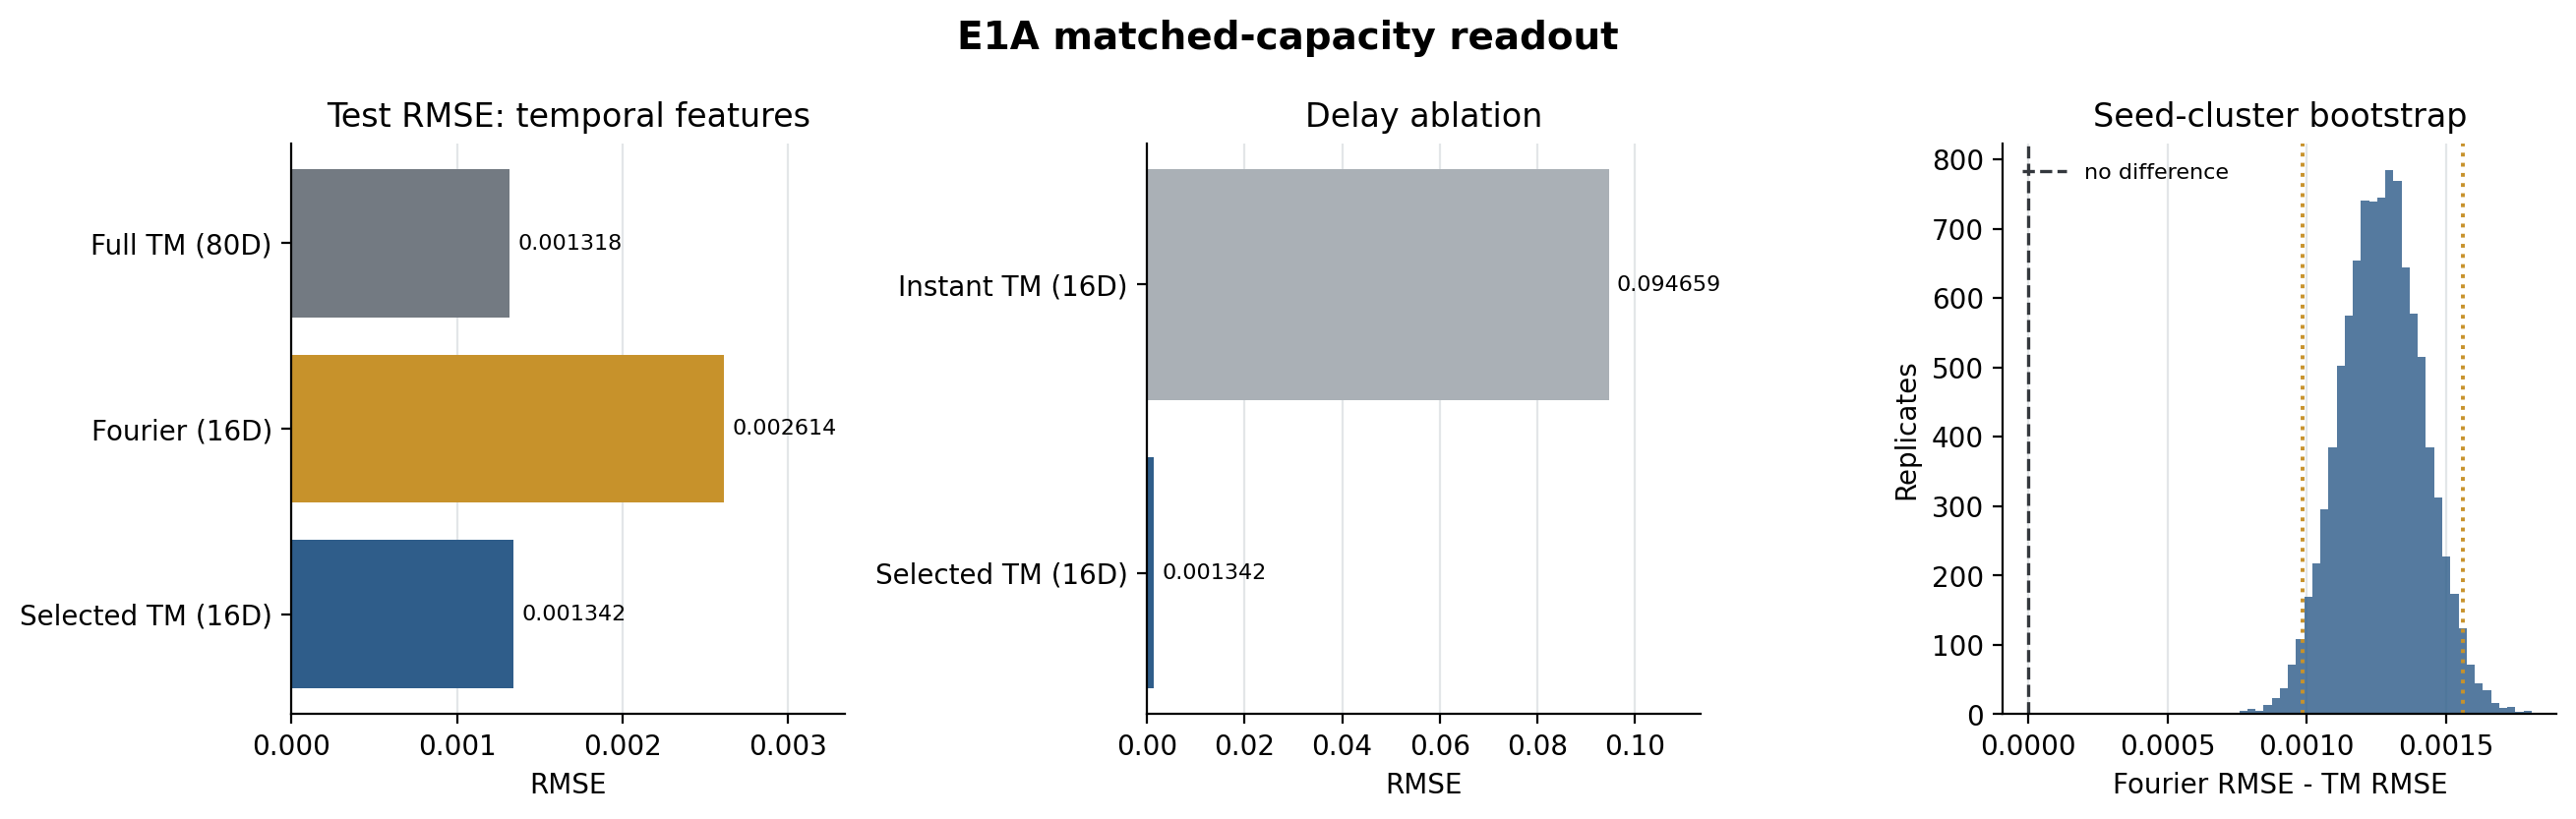
\includegraphics[width=0.96\linewidth]{../../projects/chaos-sync-thesis/experiments/runs/20260901_E1A_matched-capacity-readout/artifacts/matched_capacity_results.png}
    \caption{E1A容量一致追試。棒は新規test RMSE、bootstrap分布はFourier minus TMのseed-cluster差を示す。}
    \label{fig:e1-matched-results}
\end{figure}

この追試により、80対16という次元差だけではTM型特徴の改善を説明できない。
一方、TM側は4候補からgrouped CVで選び、Fourierの帯域定義は固定したため、
モデル選択自由度は対称ではない。また、この結果は単一写像族、補間$\alpha$、
線形ridge、有限観測長に限定される。したがって、
「この条件では凍結した短遅延TM座標が固定Fourier帯域より良かった」と結論し、
TM基底の一般的優位までは主張しない。

\subsection{E1B：2源観測の識別可能性}

E1Bでは独立な2本の一般化Boole源
\begin{equation}
    s_{j,t+1}=F_{\alpha_j}(s_{j,t}),
    \qquad j\in\{1,2\},
    \label{eq:e1b-sources}
\end{equation}
を考える。各源は式\eqref{eq:e1-standardization}と同じ中央値・半四分位幅で
個別に標準化してから混合した。この処理は周辺尺度の自明な経路を抑えるが、
未知混合の実データでは源別標準化を直接実行できないため、理想化正対照である。

full-rank観測は
\begin{equation}
    y_t=A s_t,
    \qquad
    A=\begin{bmatrix}
       1 & 0.35\\
       0.25 & 1
    \end{bmatrix},
    \qquad
    \det A=0.9125\neq0,
    \label{eq:e1b-full-rank}
\end{equation}
とした。$A$が既知なら$s_t=A^{-1}y_t$であり、観測段階では源順序を失わない。
したがって、単一源特徴写像$\Phi(\alpha)$が候補集合上で十分に識別的なら、
連結写像
\begin{equation}
    \Phi_2(\alpha_1,\alpha_2)
    =\bigl(\Phi(\alpha_1),\Phi(\alpha_2)\bigr)
\end{equation}
も順序付きパラメータを識別する。これは既知$A$のoracle正対照であり、
blind source separationの定式化ではない。

これに対し、rank-one対称観測を
\begin{equation}
    v_t
    =\frac{s_{1,t}+s_{2,t}}{\sqrt{2}}
    =\frac{1}{\sqrt{2}}
      \begin{bmatrix}1&1\end{bmatrix}s_t
    \label{eq:e1b-rank-one}
\end{equation}
とする。源とパラメータの同時入替え
\begin{equation}
    (s_1,\alpha_1)\longleftrightarrow(s_2,\alpha_2)
\end{equation}
は$v_t$を全時刻で不変にする。したがって同一観測に
$(a,b)$と$(b,a)$という異なる順序付き目標を割り当てられる。
同一観測に対する任意の決定論的予測を$p=(p_1,p_2)$とすると、
衝突2行の要素平均二乗誤差は
\begin{align}
    \mathcal L(p;a,b)
    &=\frac{1}{4}\Bigl[
      (p_1-a)^2+(p_2-b)^2
      +(p_1-b)^2+(p_2-a)^2
      \Bigr],\\
    \min_p\mathcal L(p;a,b)
    &=\frac{(a-b)^2}{4},
    \qquad
    p^{\ast}=\left(\frac{a+b}{2},\frac{a+b}{2}\right).
    \label{eq:e1b-collision-loss}
\end{align}
ゆえに衝突1組の順序付きRMSE下限は
\begin{equation}
    \RMSE_{\min}(a,b)=\frac{|a-b|}{2}.
    \label{eq:e1b-pair-floor}
\end{equation}
複数の衝突行を等重みで集約した下限は
\begin{equation}
    \RMSE_{\mathrm{floor}}
    =\sqrt{
       \frac{1}{n}
       \sum_{r=1}^{n}
       \left(\frac{\alpha_{1,r}-\alpha_{2,r}}{2}\right)^2
    }.
    \label{eq:e1b-global-floor}
\end{equation}
この下限は特徴基底や回帰器の性能ではなく、観測写像の非単射性から生じる。

\subsection{E1Bの数値実験設計}

fit $\alpha$は$\{0.34,0.42,0.50,0.58,0.66\}$の異なる2値全10組、
test $\alpha$は未使用補間点$\{0.38,0.46,0.54,0.62\}$の全6組である。
fitは16 pair seed、testは32 pair seedを用い、各unordered pairから
forwardとswappedの2行を作った。したがってfitは320行、testは384行である。
源軌道は2,048点をburn-inし、4,096点を観測した。

式\eqref{eq:matched-tm-coordinates}のTM16を再選択せず凍結し、
各源または各観測チャネルへ適用した。比較した6モデルは、
既知$A^{-1}$で源を戻すoracle TM/Fourier、2混合チャネルから直接読むTM/Fourier、
対称1チャネルから読むTM/Fourierである。
目的ベクトル$a_r=(\alpha_{1,r},\alpha_{2,r})^{\mathsf T}$に対し、
multi-output ridgeを
\begin{equation}
    (\widehat b_{\lambda},\widehat B_{\lambda})
    =\arg\min_{b,B}
      \sum_{r\in\mathrm{fit}}
      \left\|a_r-b-B^{\mathsf T}\widetilde h_r\right\|_2^2
      +\lambda\|B\|_{\mathrm F}^2
    \label{eq:e1b-multi-ridge}
\end{equation}
で学習した。$\lambda$はfit pair seedの4-fold grouped CVによる順序付きRMSEだけで選び、
testでは全要素の順序付きRMSEと、各行で目標順序を交換した小さい方を採る
permutation-invariant RMSEを記録した。

事前条件は、oracle TMのtest RMSEが0.005未満、
swapped衝突対のrank-one特徴差が$10^{-12}$以下、
rank-one TM/Fourierの順序付きRMSEが式\eqref{eq:e1b-global-floor}を下回らないことである。

\subsection{E1Bの結果と考察}

\begin{table}[htbp]
\centering
\small
\caption{E1Bのgrouped CVと新規test RMSE。PIはpermutation-invariantを表す。}
\label{tab:e1b-results}
\begin{tabular}{lrrrr}
\toprule
モデル & 次元 & CV ordered & test ordered & test PI \\
\midrule
oracle TM, full-rank & 32 & 0.002429 & 0.002083 & 0.002083 \\
oracle Fourier, full-rank & 32 & 0.003109 & 0.003051 & 0.003051 \\
direct TM, full-rank & 32 & 0.009502 & 0.007740 & 0.007740 \\
direct Fourier, full-rank & 32 & 0.011008 & 0.009070 & 0.009070 \\
direct TM, rank-one & 16 & 0.090014 & 0.073710 & 0.073710 \\
direct Fourier, rank-one & 16 & 0.090335 & 0.073891 & 0.073891 \\
\bottomrule
\end{tabular}
\end{table}

test集合に対する理論下限は
\begin{equation}
    \RMSE_{\mathrm{floor}}=0.073029674
\end{equation}
だった。rank-one TMは0.073710、Fourierは0.073891で、いずれも下限を下回らなかった。
全352衝突対におけるforward/swappedのTM/Fourier特徴最大絶対差は厳密に0だった。
一方、oracle TMは0.002083で事前閾値0.005を通過し、
direct TMも0.007740とrank-one下限より約89.4\%小さかった。
独立validatorは20項目中20項目が通過した。

\begin{figure}[htbp]
    \centering
    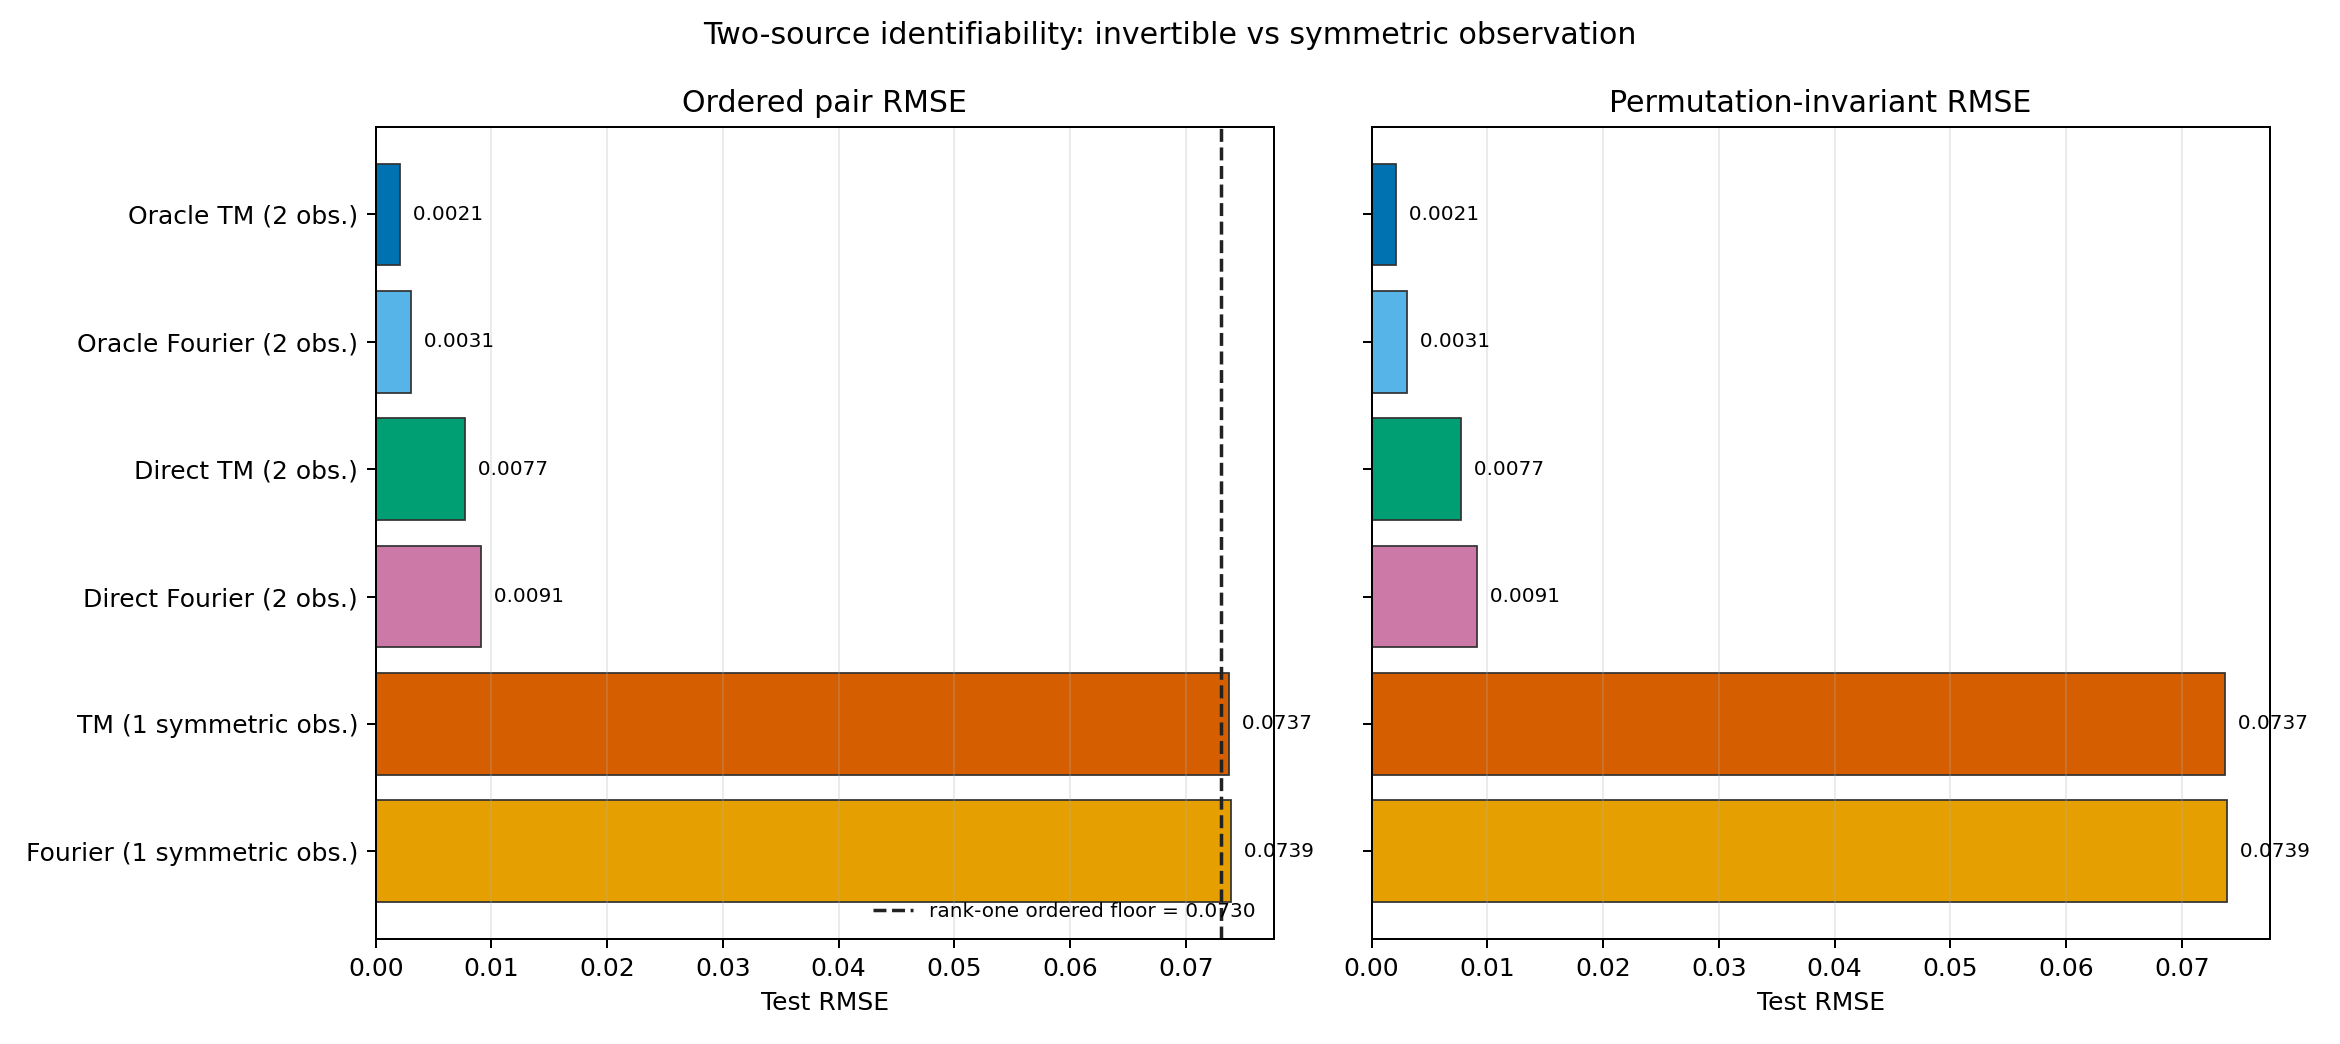
\includegraphics[width=0.98\linewidth]{../../projects/chaos-sync-thesis/experiments/runs/20260901_E1B_two-source-identifiability/artifacts/identifiability_results.png}
    \caption{E1Bのfull-rank 2観測と対称rank-one 1観測の比較。破線は順序付きRMSEの理論衝突下限である。}
    \label{fig:e1b-identifiability}
\end{figure}

この結果は、可逆2観測では凍結した有限時間特徴から順序付き2源パラメータを読める一方、
対称1観測が捨てた源順序をTM特徴が作り直すことはできない、という境界を示す。
rank-oneのPI RMSEもordered RMSEと同じだったのは、順序付き教師で学習したridgeが
衝突対の中点に近い同一2座標を返したためである。
これはunordered pair自体の識別不能を証明しない。sorted target専用probeは別実験を要する。

また、oracle条件でTMの点推定はFourierより約31.7\%、direct条件では約14.7\%小さかったが、
この差の区間推定はE1Bの事前主指標ではない。既知$A$、源別標準化、補間$\alpha$、
固定混合行列という制約もあるため、TM一般優位やblind source separationの証拠とはしない。

\section{E0からE1へ得られた研究上の結論}

E0からE1Bまでの結論は、次の五段階に整理できる。

\begin{enumerate}
    \item \textbf{理論・実装整合性：}
    単一一般化Boole写像のCauchy尺度とLyapunov指数は、保存済み実装で再現された。
    \item \textbf{有限時間情報の存在：}
    周辺尺度を抑えた後にも、時間遅延・周波数特徴から未使用$\alpha$を回収できた。
    \item \textbf{容量差だけでは説明できないTM改善：}
    16次元同士の新規testでも、選択TM短遅延は固定Fourier帯域より小さいRMSEを示し、
    差の95\% seed-cluster区間は正だった。
    ただし候補選択自由度が非対称なため、普遍的な基底優位とはしない。
    \item \textbf{観測写像の識別可能性境界：}
    可逆2観測では順序付き2源パラメータを回収できたが、
    対称1観測では源入替えの完全衝突から式\eqref{eq:e1b-global-floor}の誤差下限が生じた。
    \item \textbf{同期・圧縮は未検証：}
    E0--E1Bはいずれも読み出し前段の検証であり、同期による自由度縮約、
    符号長、rate--distortion、画像復号を評価していない。
\end{enumerate}

次の読み出し実験E2Aでは、E1Bの混合行列、split、特徴、probe選択法を固定し、
観測ノイズ強度だけを変える。観測
\begin{equation}
    y_t^{\mathrm{obs}}=A s_t+\eta_t,
    \qquad
    \eta_t\sim\mathcal N(0,\sigma^2 I),
\end{equation}
に対し、oracle逆変換後のノイズ共分散は
\begin{equation}
    \operatorname{Cov}(A^{-1}\eta_t)
    =\sigma^2 A^{-1}A^{-\mathsf T}
\end{equation}
となる。この誤差増幅を理論予測として、どのSNRで順序付き復号が崩れるかを測る。
行列条件数の走査はノイズ強度を固定した後の別実験とする。
なお、結合系の同期転移を扱うE3Aは別系列であり、本ノートの読み出し結論と混同しない。

\section{再現ファイル}

本ノートの数値は、次の保存成果物から転記した。

\begin{itemize}
    \item E0：\path{projects/chaos-sync-thesis/experiments/runs/20260806_E0_boole-invariant-measure/}
    \item E1A pilot：\path{projects/chaos-sync-thesis/experiments/runs/20260830_E1A_temporal-alpha-readout/}
    \item E1A追試：\path{projects/chaos-sync-thesis/experiments/runs/20260830_E1A_temporal-alpha-replication/}
    \item E1A容量一致：\path{projects/chaos-sync-thesis/experiments/runs/20260901_E1A_matched-capacity-readout/}
    \item E1B 2源識別可能性：\path{projects/chaos-sync-thesis/experiments/runs/20260901_E1B_two-source-identifiability/}
\end{itemize}

各runにはconfig、使用データまたは決定論的由来、モデル入力NPZ、test予測、
seed別・条件別CSV、プロットと元表、実行コード、環境、SHA-256、独立validatorを保存した。
本ノートの表は各runの\path{artifacts/summary.json}またはCSVから転記している。

\begin{thebibliography}{9}
\bibitem{umeno2016}
K. Umeno and K.-i. Okubo,
``Exact Lyapunov exponents of the generalized Boole transformations,''
\textit{Progress of Theoretical and Experimental Physics}, 2016, 021A01, 2016.

\bibitem{umeno2026}
K. Umeno,
``Infinite Dimensional Chaotic Synchronization for Randomly Coupling Systems and Dynamical Phase Transition,''
preprint, July 5, 2026.
\end{thebibliography}

\end{document}
